\chapter{Background}
This chapter provides the necessary background for understanding the problem of write amplification in B-trees and the proposed method by outlining the characteristics of external storage, the architecture of database systems, and the behavior of B-trees in out-of-memory environments. 
Furthermore, it introduces the concepts of write, read, and space amplification, which allow for a differentiated analysis of index structures for their efficiency and performance characteristics.

\section{External Storage Characteristics}
For some time, in-memory database systems like Hyper \cite{kemper2011hyper} have gained popularity due to the decreasing cost of \ac{DRAM}.
However, that trend has reversed recently, as \ac{DRAM} prices have stagnated \cite{haas2023modern} and \ac{SSD} price-performance-ratios have improved significantly \cite{leis2024leanstore}.
Therefore, modern database systems are designed to operate efficiently on external storage and since index structures are the performance-critical component, out-of-memory indexing has become a key consideration again.
B-trees have been the dominant index structure for out-of-memory indexing, since their high fanout minimizes the number of \ac{IO} operations.

Historically, hard disks were the dominant storage medium.
Hard disks have a significant imbalance in latency between random and sequential \ac{IO} due to their mechanical nature.
While \ac{SSD} have a smaller difference between random and sequential \ac{IO}, they still exhibit asymmetric performance, especially in writes \cite{haas2023modern}.
Therefore, to amortize the cost of random \ac{IO}, database systems and their index structures are designed to access data in pages of multiple kilobytes instead of individual tuples.
This assumes that subsequent accesses exhibit some locality, which is often the case in practice.
While we will be referencing disk-based systems throughout this thesis, we speak of systems operating on external storage, which can be either disk-based or flash-based.

\section{Database System Architecture Overview}

% TODO: Mention that we don't consider writes to the log which should be the same in all systems.
% TODO: Work in equations and read/space ampl. from "A Comparison of Fractal Trees to Log-Structured Merge (LSM) Trees" https://www.cs.cmu.edu/~dga/papers/sigmod10-fractal.pdf

\begin{figure}[htpb]
  \centering
  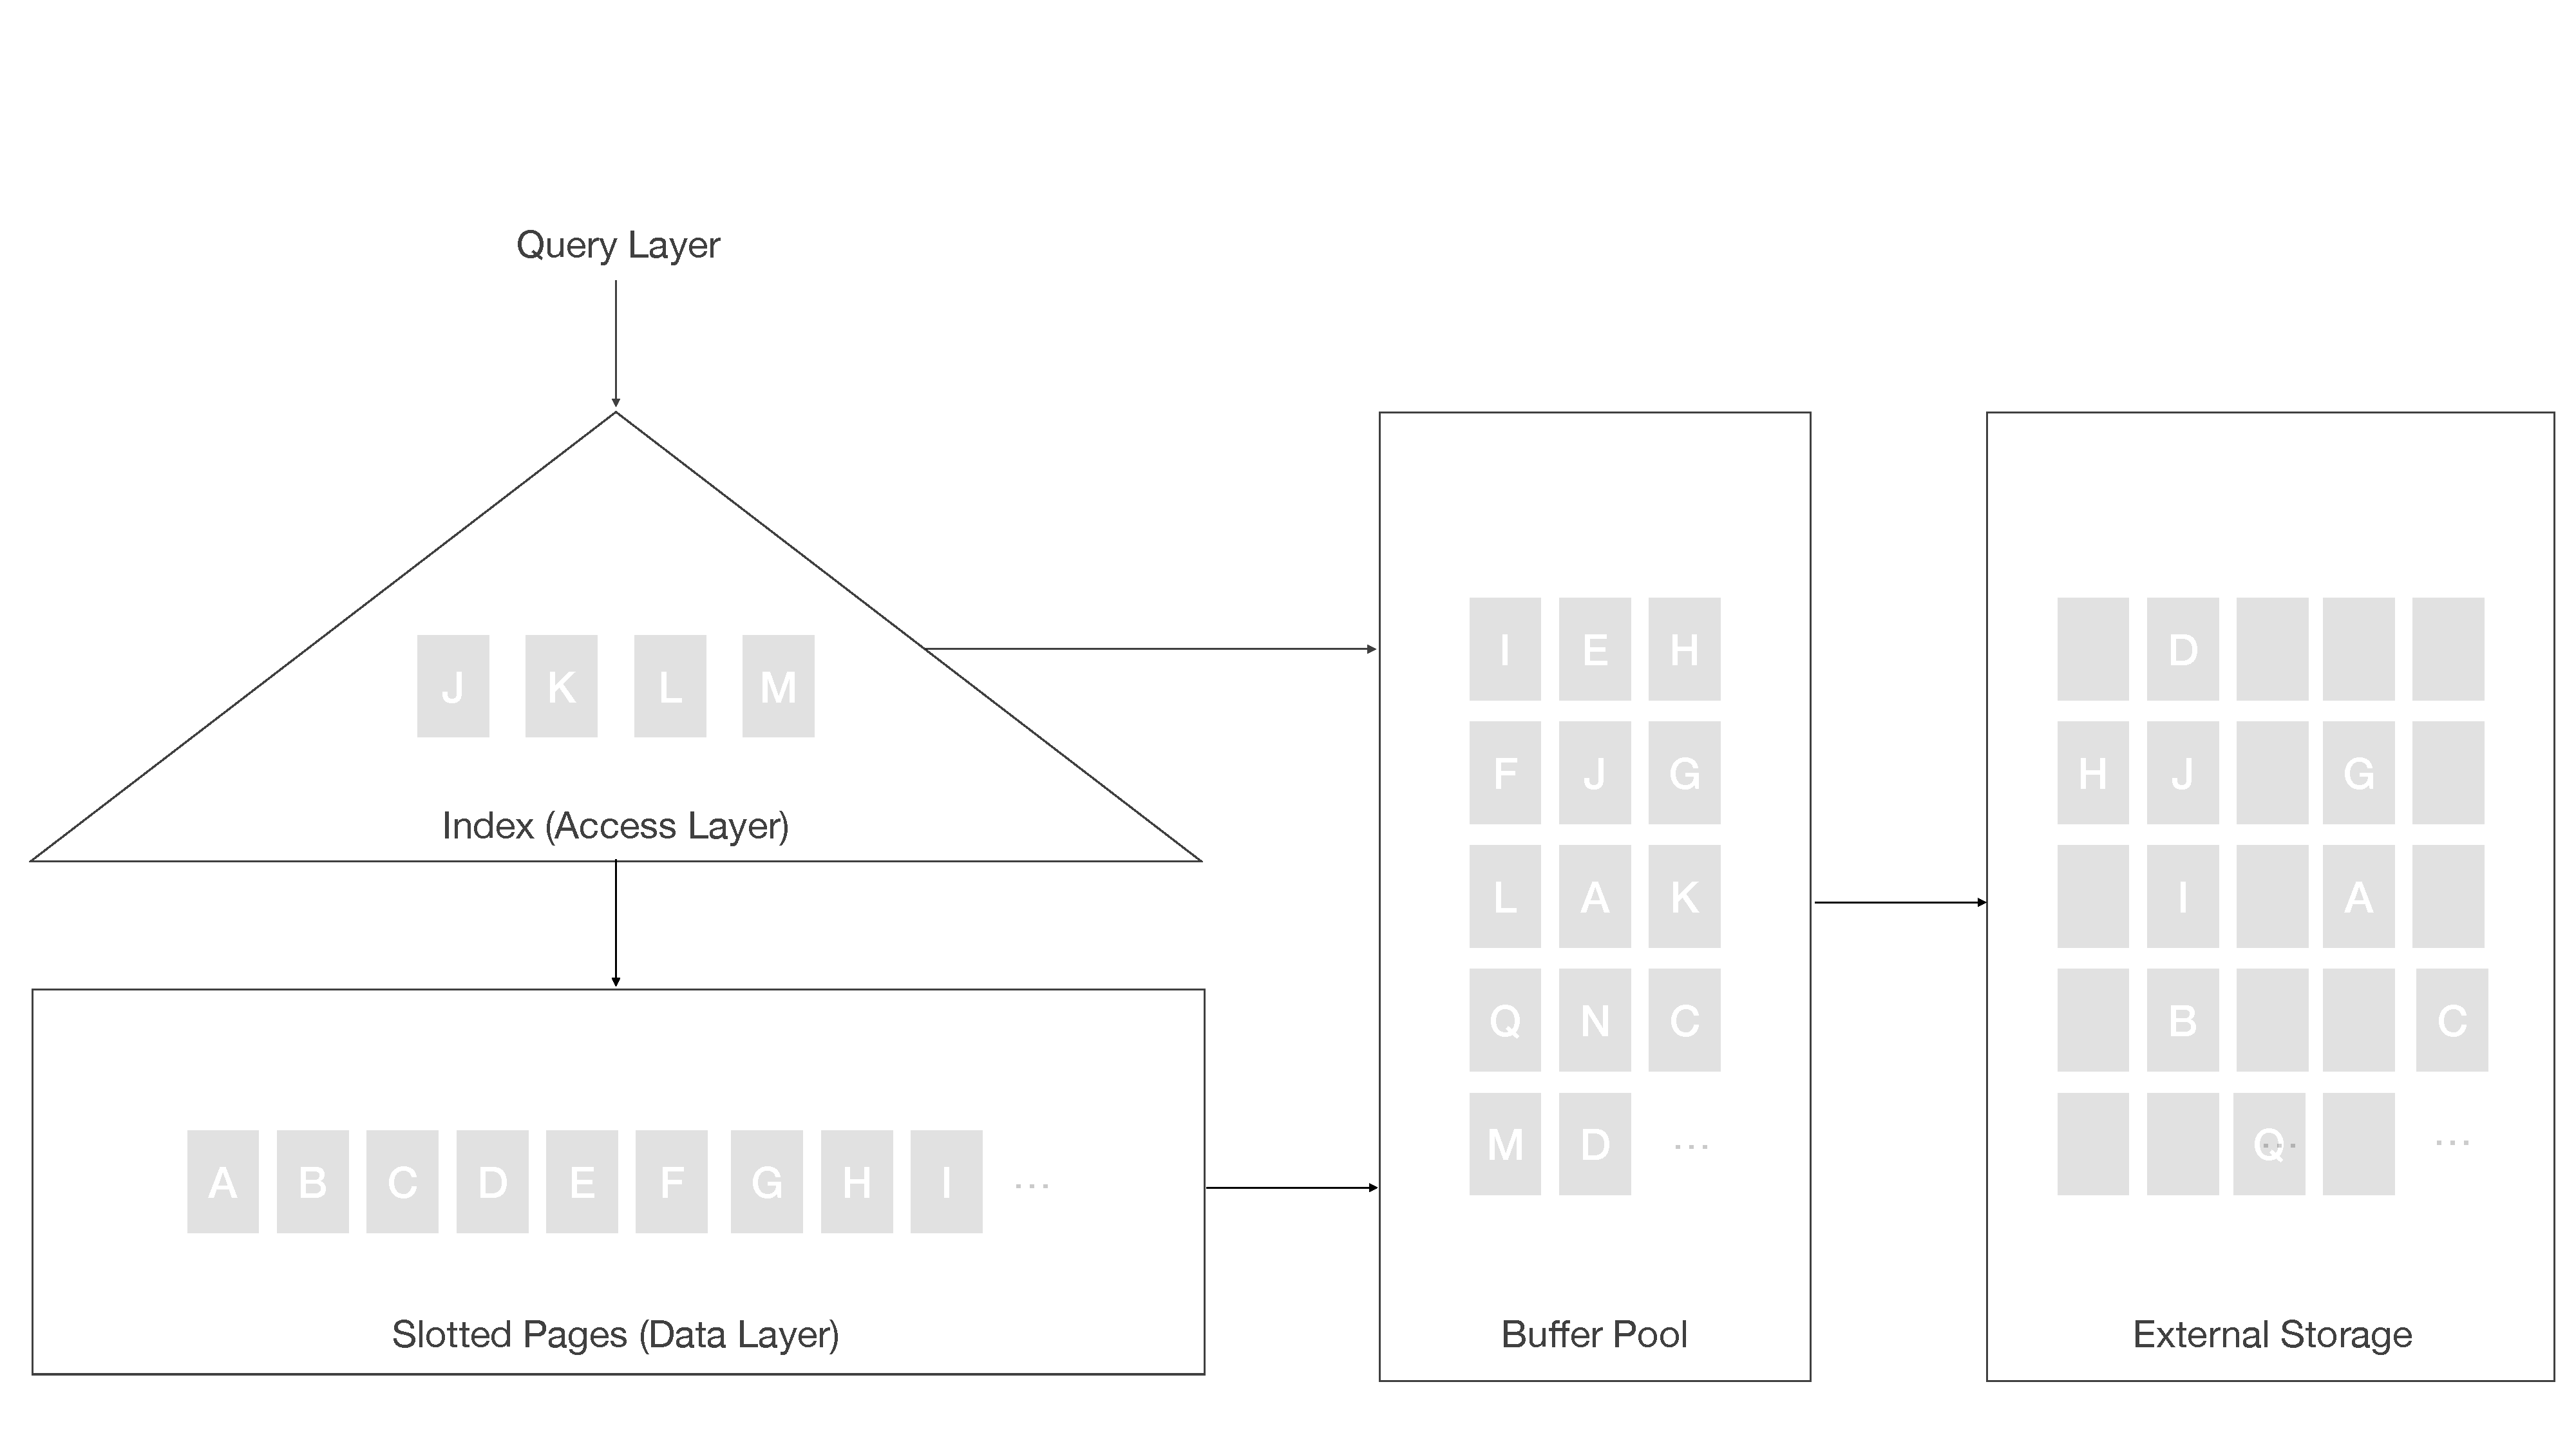
\includegraphics[width=0.99\textwidth]{figures/db_architecture.pdf}
  \caption{The storage and access layer of a database system. The index provides access to the tuples stored in the slotted pages. Each component requests data from the buffer manager, which handles caching and loading pages from external storage. Adapted from "Database Systems on Modern CPU Architectures" \cite{mdbs2024slides}.}
  \label{fig:db-architecture}
\end{figure}

In the scope of this thesis we focus on a classic architecture of a single-node, disk-based database system.
Note that this architecture is not a constraint of our method, which can be applied to any database system using B-trees as an index structure.
However, for clarity, we describe our method in the context of this architecture.

The access and storage layer of a database system typically consist of a buffer manager, one or more index structures and the slotted pages that store tuples identified by \ac{TID}s, as illustrated in \autoref{fig:db-architecture}.
Since we operate in a beyond memory setting, the buffer manager is responsible for caching pages in \ac{DRAM} and loading them from external storage when needed.
Therefore, all components accessing physical data interact with the buffer manager to load and store their pages.
When a query is executed, the index is accessed by a given key (e.g. the primary key) to find the \ac{TID} of the relevant tuple.
The index is typically stored in pages, which are loaded into the buffer pool by the buffer manager.
Using the \ac{TID}, the corresponding tuple can be retrieved from the slotted pages.
The \ac{TID} encodes the \ac{PID} and the slot number within the page.
When a tuple is updated, the corresponding page is loaded into the buffer pool, modified, and marked as dirty.
Should the buffer pool be full, the buffer manager evicts pages based on its replacement policy.
Clean, unchanged pages can be discarded, while dirty, modified pages must be written back to external storage.

\section{Index Structures}
Index structures are data structures that enable efficient access to data stored in a database.
Typically, they map a key to a constant, unique \ac{TID}.
Ideally, the \ac{TID} nevers changes, as this would require all indexes pointing to that tuple to be updated.
Keys can be arbitrary types and therefore of fixed or variable size, such as integers or strings.
We will consider both within this thesis.
When the key of a tuple changes, the index must be updated to reflect the new key.

Some key-value stores directly map keys to tuples within their index structure, omitting the indirection via \ac{TID} and slotted pages.
However, in a general purpose \ac{DBMS}, we typically want to support multiple indexes on the same data.
If we stored tuples directly in the index, we would need to update all indexes when a tuple changes.
Therefore the access and storage layer are decoupled via \ac{TID}s.
For the context of this thesis, however, it does not matter whether the index maps keys to \ac{TID}s or directly to tuples.

Indexes can be classified into primary and secondary indexes.
A primary index is built on the primary key of a table, which uniquely identifies each tuple.
A secondary index is built on a non-primary key, which can be non-unique.

Consider the following example use-case: a user database with a primary key on the user ID and a secondary index on the email address.
When inserting several new users, we update the indices.
The primary index is updated with an auto-incrementing user ID, thus, the primary key follows a sequential access pattern.
However, the email addresses of new users are likely to be random and not follow any specific order.
Therefore, if the secondary index is sorted on the keys, as they are in a B-tree, the index exhibits a random access pattern.
Such access patterns have implications on the performance of index structures, as we will discuss in the following sections.

% TODO: SSD Wear Leveling? Garbage Collection? Wearout? https://www.vldb.org/pvldb/vol18/p4295-haas.pdf

\section{B-trees}

\begin{figure}[htpb]
  \centering
  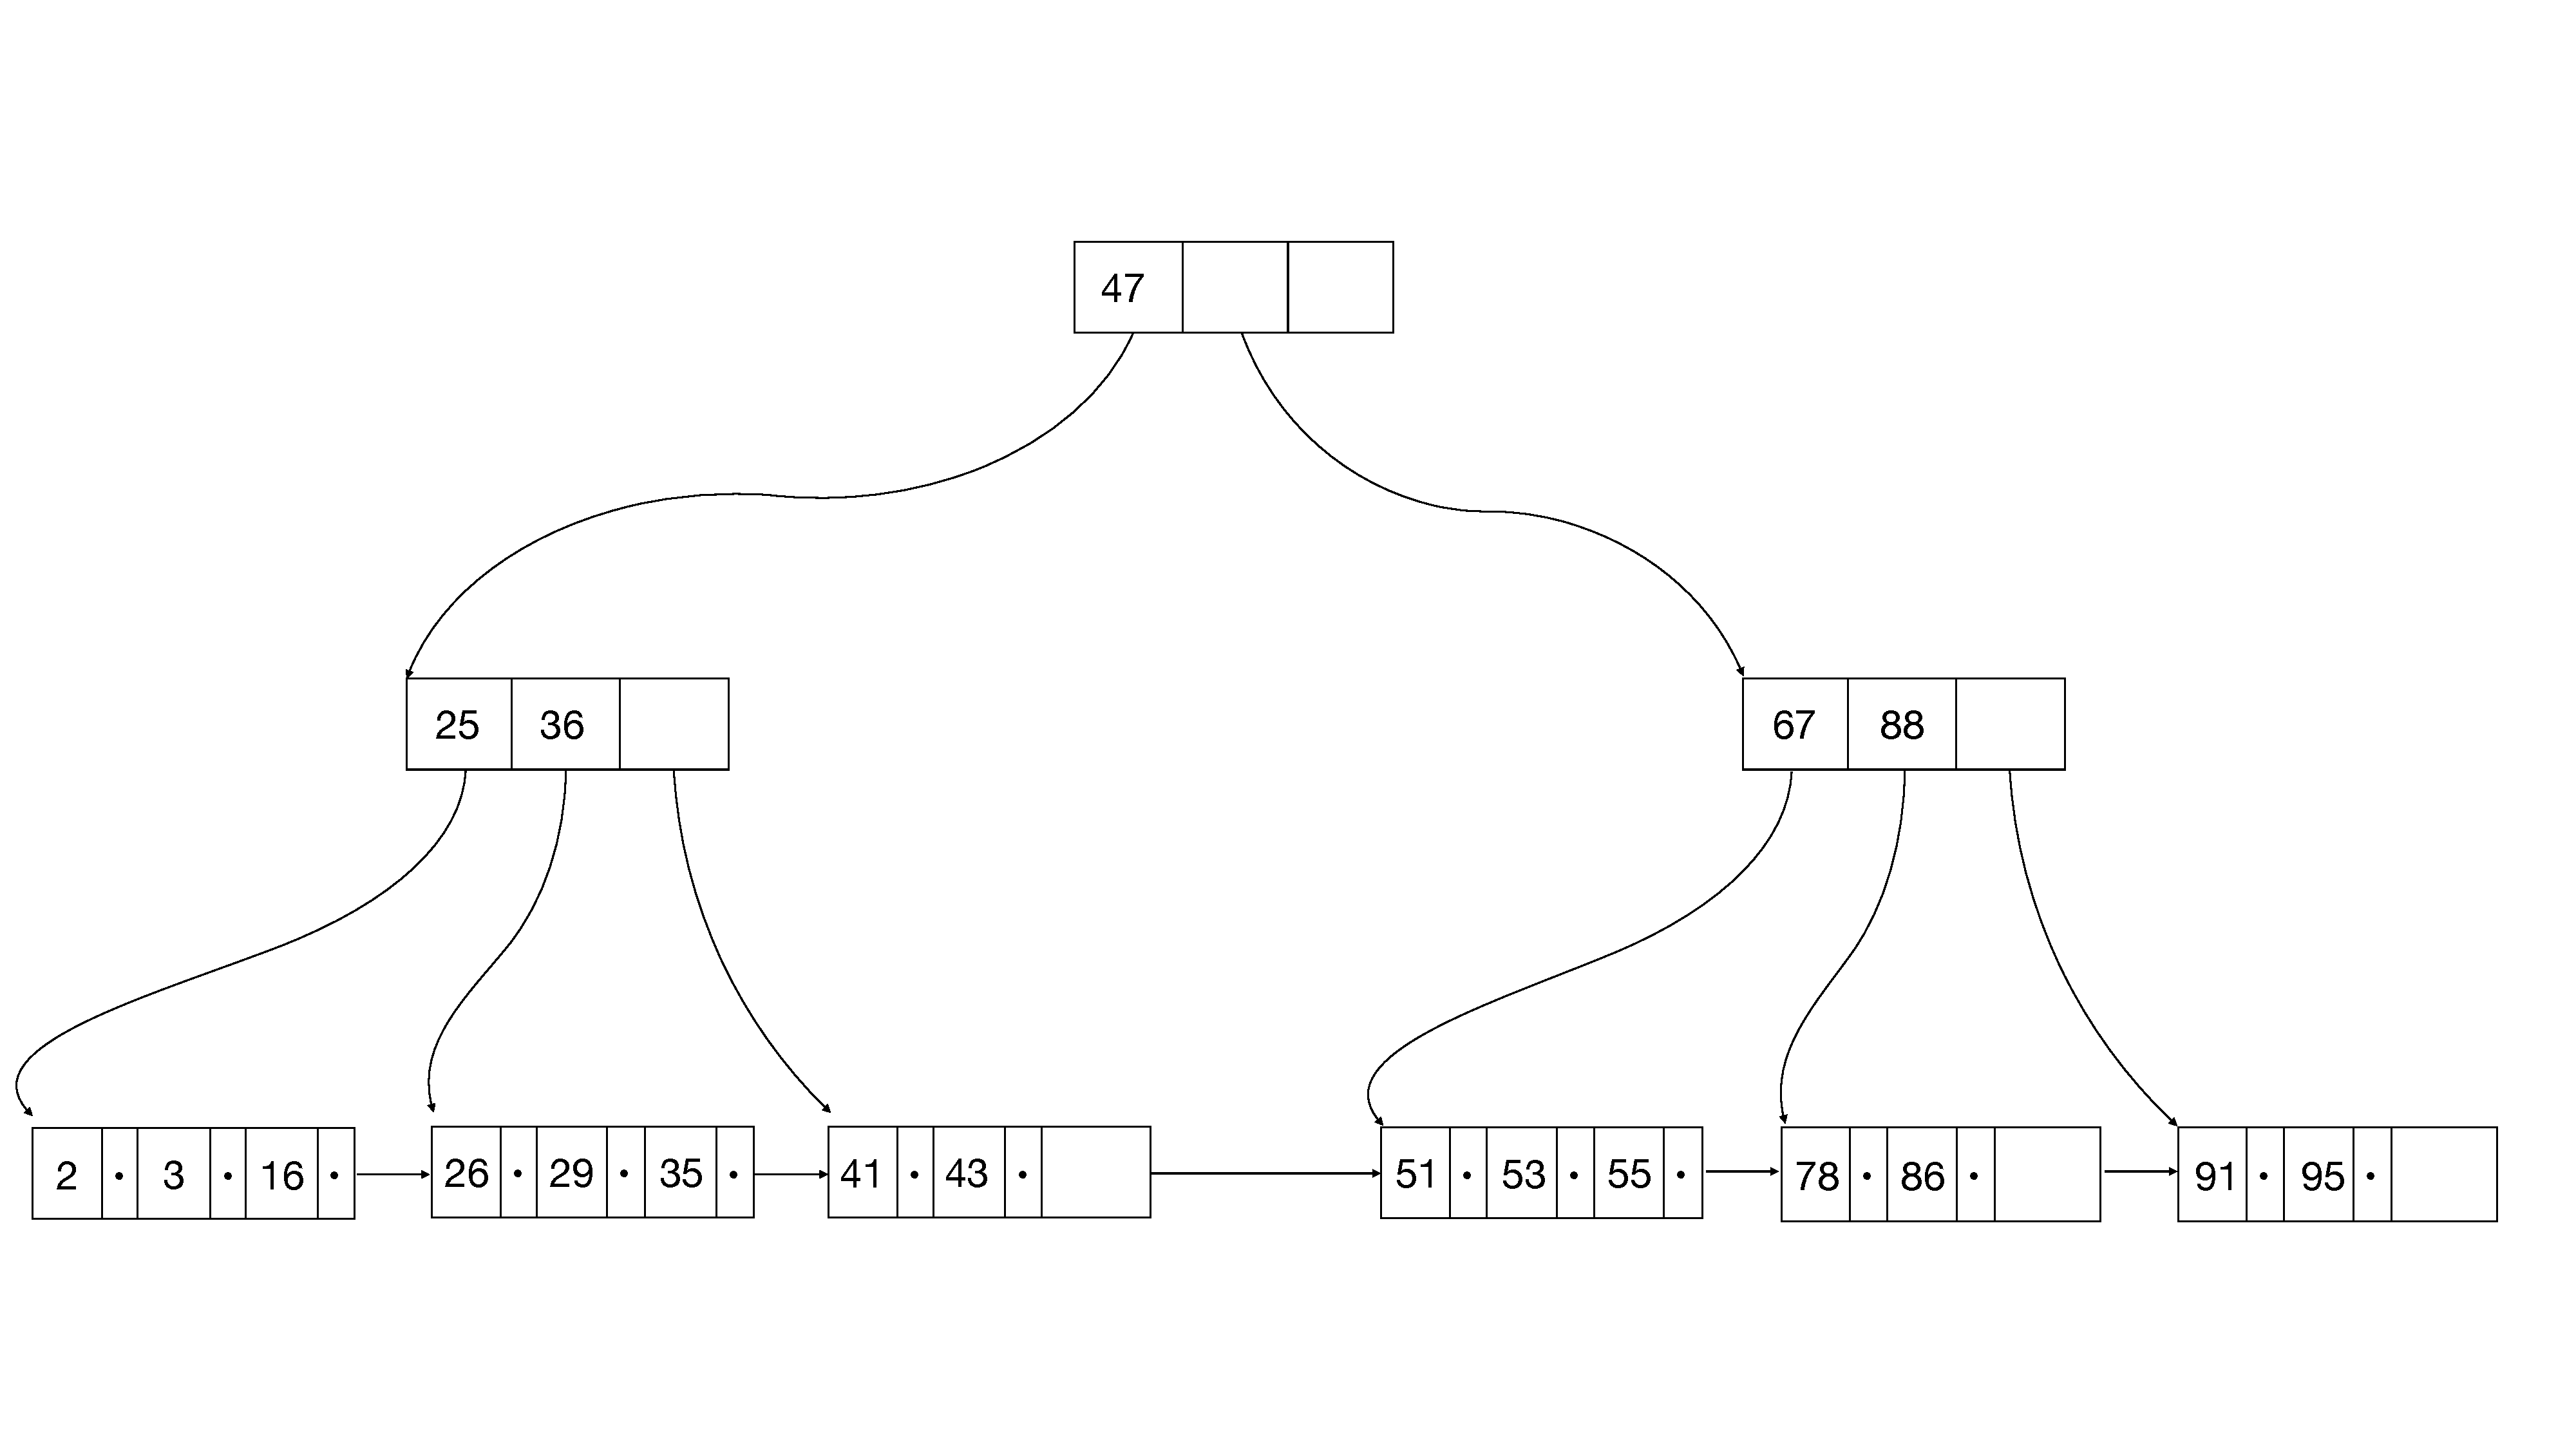
\includegraphics[width=0.99\textwidth]{figures/b_tree.pdf}
  \caption{A B+-Tree. Child pointers are represented as arrows. Values (the \ac{TID}) are represented as bullet points •.}
  \label{fig:B-tree}
\end{figure}

B-trees \cite{bayer1970organization} are a self-balancing tree data structure that maintains sorted data and allows for insertion, deletion, and search operations in logarithmic time, $\mathcal{O}(\log n)$, where $n$ is the number of entries in the tree.
A B-tree is organized in fixed-size pages, called nodes. These pages are transferred and cached transparently by the buffer manager between external storage and \ac{DRAM}.
Each node can split off a sibling once it is full. If a node is full and a new key needs to be inserted, the node splits into two nodes, and the middle key is promoted to the parent node.
Additionally, nodes can merge with a sibling if they become less than half full. For simpliticity, we omit merging of nodes in this thesis.

The tree only increases in height when the root node splits.
Each node contains between 2 and 2k entries, except for the root node, which can contain between 1 and 2k entries.
Each entry is a triple of a key, a pointer to a child node, and optionally a value (the \ac{TID}).
The entries in each node are sorted by key. On leaf nodes (nodes without children), the pointer to a child node is undefined.
An inner node (a node that is not a leaf) with k keys has k+1 children.
Each entry in an innder node separates the key space of its children.
The additional child pointer is necessary to separate the key space above the largest key in the node.
For example, consider an inner node with keys \{10, 20, 30\}.
The first child contains all keys less than 10, the second child contains all keys between 10 and 20, and the third child contains all keys between 20 and 30. 
The fourth child contains all keys greater than 30.

When searching for a key in the tree, we start at the root node.
On each node, we perform a binary search to find the appropriate pivot key and follow the corresponding child pointer.
We stop when we reach a node with the desired key.

\subsection*{B+-Trees}
When addressing B-trees in this thesis, we actually refer to B+-Trees, a variant of B-trees where all values are stored in the leaf nodes and internal nodes only store keys and child pointers to guide the search.
The separator keys in internal nodes may or may not occur in the data. An example B+-Tree is illustrated in \autoref{fig:B-tree}.
The lookup procedure is the same as in a B-tree, however we always traverse the full tree from root to leaf to find a key.
Not only does this simplify the B-tree logic, it also increases the fanout of inner nodes, leading to a lower tree height and therefore fewer \ac{IO} operations for lookups since less pages are involved in reaching the leaf level.
Also, it allows for efficient range queries by scanning the leaf nodes in order.
Due to its excellent lookup performance, support for range queries, and simplicity, B+-Trees are the dominant data structure for external storage \cite{mdbs2024slides}.

% TODO: Cut this subsection?
\subsection*{Disk-Access-Model}
To analyze the performance of B-trees in a beyond memory setting, we use the \ac{DAM} \cite{aggarwal1988complexity} \cite{kuszmaul2014fractal}.
The model has two levels of memory: an internal memory of size $M$ and external storage of infinite size.
The storage device is organized in fixed-size pages, which are the units of data transfer between memory and storage and determine the size of nodes in a B-tree.
For simplicity of this analysis of the \ac{DAM} for B-trees, we assume that records are constant sized (An assumption that simplifies this explanation but does not hold in practice. 
Therefore we will \textbf{not} assume this in our method and implementation.) and that nodes are always completely filled.
When a database has $N$ records, and the storage device has pages of size $P$, the B-tree has a height of $\log_P(N/P)$, where inner nodes contain $O(P)$ children and leaf nodes contain $O(P)$ records.

Each lookup/insertion/deletion requires a traversal from the root to a leaf node, leading to $\mathcal{O}(\log_P(N/P))$ \ac{IO} operations.
Since the majority of nodes in the tree are leaf nodes, we can assume that most inner nodes can be cached by the buffer manager.
In that case, we would require only a single \ac{IO} per B-tree operation.

In practice, B-trees are often used to index variable-sized keys and values.
Therefore, we will consider variable-sized records in our method and implementation.
However, the \ac{DAM} provides an approximation.

% TODO: Slotted Node Layout here or in Implementation?

\subsection*{Node Size \& Fanout}
\label{sec:node-size-fanout}
The node size (i.e. the page size) is a crucial parameter in the design of a B-tree, as it affects the height of the tree.
Larger nodes lead to more entries per node, increasing the fanout for inner nodes and decreasing the height of the tree.
When we can address more children per node, we need fewer levels in the tree to address the same number of keys.
Since every lookup/insert/delete operation requires a traversal from the root to a leaf node, fewer levels lead to fewer pages involved in the lookup.
Thus, larger nodes lead to fewer \ac{IO} operations per lookup.
Additionally, since we need fewer distinct pages, we induce less page management overhead in the buffer manager.

Large nodes are particularly beneficial for analytical, read-heavy workloads, which often perform large scans and are interested in large parts of the data.
However, workloads that perform many updates and point queries, are sometimes only interested in a small portion of the page.
As a result, larger nodes lead to more \ac{IO} amplification, as we read and write significantly more data than necessary to perform the operation.
If subsequent operations follow a sequential access pattern, the \ac{IO} amplification is not a problem, as we will be operating on pages already cached by the buffer manager.
Ideally, no or very few additional \ac{IO} operations are necessary.
With random access patterns, however, this \ac{IO} amplification due to large page sizes becomes a problem.
% Modern \ac{SSD} were shown to perform best at page sizes of 4 KB \cite{haas2023modern}.

% TODO: Make sure this is still correct by the end of the thesis:
While we will be evaluating performance under different node sizes, this tuning parameter is not the primary focus of this thesis.
Instead, we focus on reducing \ac{IO} amplification in B-trees at any page size.
However, larger nodes are expected to profit more significantly from our approach, as they induce more \ac{IO} amplification in B-trees.


\section{Write Amplification}
Write amplification is the ratio of the amount of data written to storage versus the amount of logical data written by the user.
For example, if the database updates an entry of 64 B, but needs to write a full page of 4 KB to storage, the write amplification is 4096 B / 64 B = 64.
Write amplification $WA$ is formally defined as:

\[
WA = \frac{Bytes Written Physically}{Bytes Written Logically}
\]

There are multiple layers of write amplification in a database system, which we need to differentiate from each other.

\inlinesection{Application Layer.}
At the application layer, we consider an external end user interacting with the database system, e.g. through SQL.
When an end user inserts a tuple through a query, the database system must insert the tuple in the table itself, in the \ac{WAL} and all indexes that serve to access the tuple later.
Consequently, we write significantly more bytes than the user requested logically.
Additionally, updating a B-tree index might cause structural changes such as node splits or merges that create new nodes, delete new nodes and update the parent nodes.
Thus, a database system inherently comes with write amplification merely to perform its purpose: manage data.
This is not the focus of this thesis; we consider all updates to tables, data structures and the \ac{WAL} as necessary and focus on reducing write amplification within the index layer specifically.

% TODO: We kinda do measure write amplification on this layer as well as bytes inserted not "B-Tree" as the user.
\inlinesection{Index Layer.}
At the index layer, we consider the B-tree as the user of pages.
When a B-tree entry is updated, the bytes written logically include not only the updated key but also any additional metadata required to maintain the tree structure.
This can include information about node splits, merges, and the promotion of keys to parent nodes.
The writes are amplified by the B-tree's page structure that requires rewriting the entire page even if only a small portion has changed.
As mentioned in \autoref{sec:node-size-fanout}, the node size directly impacts the write amplification at this level.
This is the write amplification we focus on in this thesis, by minimizing the number of pages written to storage for a given set of updates (see \autoref{chap:method}).

\inlinesection{Physical Layer.}
At the physical layer, we consider the database system as the user (the host) of the physical storage device.
When the database system writes a page to storage, the bytes written logically are the size of the page.
However, due to the characteristics of the storage device, the actual bytes written physically can be larger.
\ac{SSD} typically operate in larger units called blocks, which consist of multiple pages.
When a page is updated, the entire block containing that page must be rewritten, leading to write amplification.
Additionally, when garbage collection is performed, valid pages within a block must be copied to a new block before the old block can be erased and reused.
Recent research observed write amplification factors up to 10x on modern \ac{SSD} \cite{haas2025ssd}.
Consequently, a page write of 4 KB can lead to physical writes of up to 40 KB on the device, using up valuable bandwidth and wearing out the device faster.
While we do not focus on hardware-level write amplification in this thesis, it shows the importance of reducing write amplification at the host level.
Unnecessary writes by the database system are multiplied by \ac{SSD}.

% See Bepsilon paper for more analytical model

% TODO: We kina misuse this term in the evaluation chapter, since we do count the reads, not the total IO upon one read.
\section{Read Amplification}
Read amplification is the number of \ac{IO} operations required to answer a query \cite{kuszmaul2014fractal}.
As described above, a B-tree lookup requires a traversal from the root to a leaf node, which is $\mathcal{O}(\log_P(N/P))$ \ac{IO} operations in the \ac{DAM}, assuming that our cache is cold.
In practice, the buffer manager caches pages in \ac{DRAM}, which can significantly reduce the number of \ac{IO} operations.
To answer range queries, we can scan the leaf nodes in order, which is efficient in B+-Trees.
Therefore, we only traverse the tree once to find the start of the range and then scan the leaf nodes sequentially.
Read amplification is a common tradeoff when reducing write amplification, as we will see in alternative data structures (see \autoref{chap:related-work}).
We will analyze the introduced read amplification of our method compared to the traditional B-tree in our evaluation (see \autoref{chap:evaluation}).

\section{Space Amplification}
Space amplification is the ratio of the amount of space used by the data structure versus the amount of logical data stored \cite{kuszmaul2014fractal}.
Most nodes in a B-tree are leaf nodes, which store the actual data.
However, inner nodes only store keys and child pointers to guide the search, inflating the space usage.
Additionally, B-tree nodes are not always completely filled.
Therefore, B-trees exhibit some space amplification.
Space amplification is not the focus of the thesis, however we will analyze space utilization of our method compared to the traditional B-tree in our evaluation (see \autoref{chap:evaluation}).